
% Slideshow, written by Brent Baccala, for a lecture at Catholic University

\documentclass{beamer}
\usetheme{Madrid}

\title{Double Pendulum}
\author{Brent Baccala}
\institute{\tt cosine@freesoft.org}
%% \date{February 8, 2023}

\setbeamertemplate{footline}{}
\beamertemplatenavigationsymbolsempty

\usepackage{xcolor}
\usepackage{comment}
\usepackage{graphicx}

\usepackage{tabularx}

\begin{document}


\begin{frame}
\titlepage
\begin{block}{Abstract}
The Double Pendulum
\end{block}
\end{frame}

\begin{frame}
\begin{exampleblock}{}
\begin{center}
\vskip 20pt
\Huge
Part 1: The Double Pendulum
\vskip 6pt
\ 
\end{center}
\end{exampleblock}
\end{frame}

\begin{frame}
\frametitle{Free Body Diagram}
%% 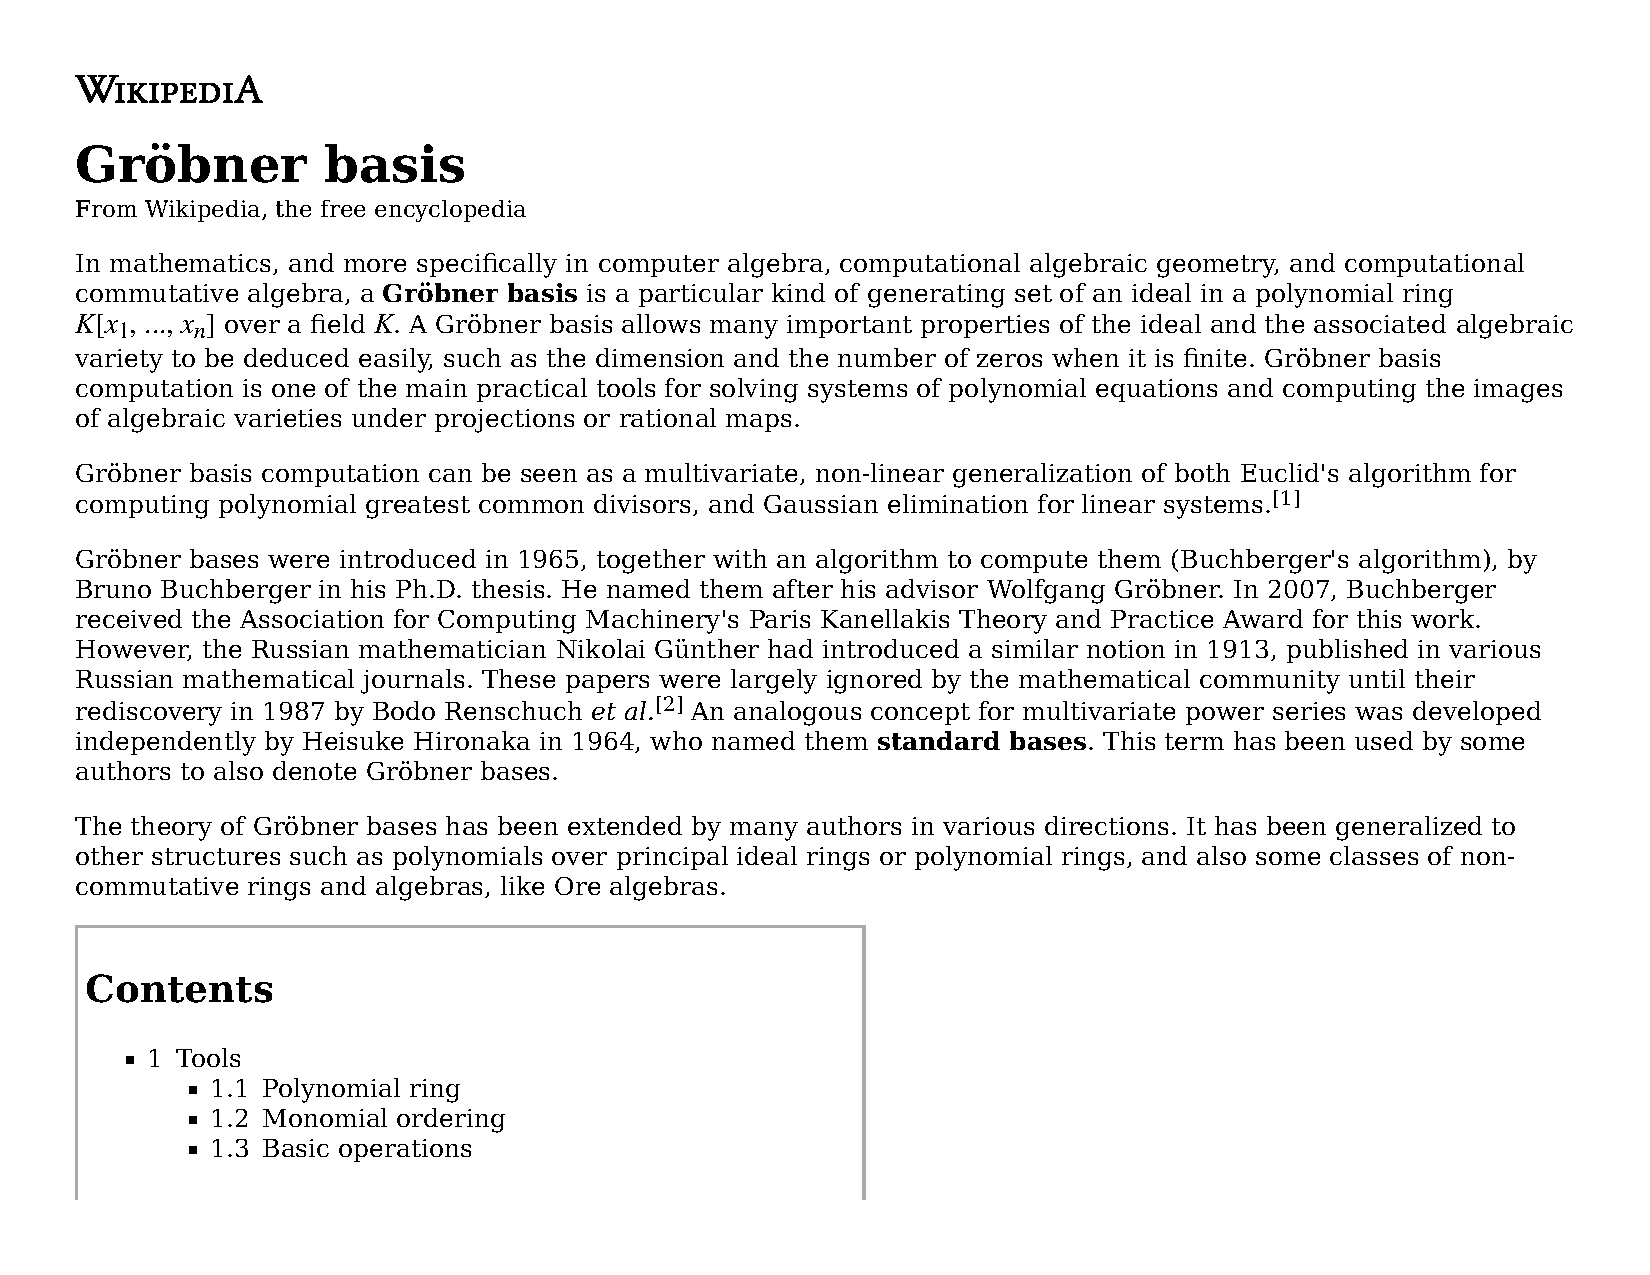
\includegraphics[clip, trim=0in 5.6in 0in 0.75in, width=\textwidth, page=1]{GrobnerBasis.pdf}
%% \includegraphics[clip, trim=0in 6.25in 0in 0.5in, width=\textwidth, page=9]{GrobnerBasis.pdf}
%% \includegraphics[clip, trim=0in 3in 0in 0.5in, width=\textwidth, page=13]{GrobnerBasis.pdf}
\end{frame}

\begin{frame}
\frametitle{Energy Calcuation}
\end{frame}

\begin{frame}
\frametitle{Lyapunov Stability}
\end{frame}

\begin{frame}
\frametitle{Flip Time}
%% \includegraphics[clip, trim=0in 5.4in 0in 0.5in, width=\textwidth, page=13]{LU decomposition - Wikipedia.pdf}
{\tiny Source: Wikipedia}
%%{\tiny Source: @MathType on Twitter}
%%\includegraphics[clip, trim=0in 2.7in 0in 0in, width=\textwidth]{LU.jpeg}

\end{frame}

\begin{frame}
\frametitle{Effect of Mass Ratio}
\end{frame}

\begin{frame}
\frametitle{Stability of the Solar System}
\end{frame}


\begin{frame}
\begin{exampleblock}{}
\begin{center}
\vskip 20pt
\Huge
Part 2: Use of the Pendulum to Measure Gravity
\vskip 6pt
\ 
\end{center}
\end{exampleblock}
\end{frame}

\begin{frame}
\frametitle{Use of the Pendulum to Measure Gravity}
\begin{itemize}
\item Importance (and difficulty) of Length
\end{itemize}
\end{frame}

\begin{frame}
\frametitle{Piezoelectronics}
\end{frame}

\end{document}
